\documentclass{article}


% to compile a camera-ready version, add the [final] option, e.g.:
\usepackage[final]{neurips}

% to avoid loading the natbib package, add option nonatbib:
    % \usepackage[nonatbib]{neurips_2019}

\usepackage[utf8]{inputenc} 	% allow utf-8 input
\usepackage[T1]{fontenc}    		% use 8-bit T1 fonts
\usepackage{hyperref}       		% hyperlinks
\usepackage{url}            		% simple URL typesetting
\usepackage{booktabs}       		% professional-quality tables
\usepackage{amsfonts}       		% blackboard math symbols
\usepackage{nicefrac}       		% compact symbols for 1/2, etc.
\usepackage{microtype}      		% microtypography
%\usepackage{breqn}			% dmath
\usepackage{listings}
\usepackage{amsmath}     		% multiline
\usepackage{graphicx}
\usepackage{xepersian}
\usepackage{graphicx}



\settextfont{XB Niloofar.ttf}

\title{پاسخ تمرین سری ۱ }




\author{%
  محمدرضا عزیزی\\
  ۹۸۱۳۱۰۲۲ \\
  دانشکده مهندسی کامپیوتر\\
  دانشگاه صنعتی امیرکبیر (پلی‌تکنیک تهران)\\
  \texttt{mrazizi@aut.ac.ir} \\
}


\renewcommand{\baselinestretch}{1.5} 

\begin{document}


\begin{minipage}{0.1\textwidth}% adapt widths of minipages to your needs

\includegraphics[width=1.1cm]{aut_logo.png}
\end{minipage}%
\hfill%
\begin{minipage}{0.9\textwidth}\raggedleft
دانشگاه صنعتی امیرکبیر (پلی‌تکنیک تهران)\\
شبکه‌های عصبی (بهار ۱۳۹۹)\\
\end{minipage}
% \end{}


\makepertitle




% 1
\section{
راهکاری برای پیش‌پردازش داده‌ها
}

داده‌ها با استفاده از کتابخانه pandas بارگذاری کرده و از آن‌جایی که ستون‌های داده‌ها نام ندارد، ابتدا با توجه به توضیحات دیتاست، یک لیست برای نام ستون‌ها تعریف کرده و این نام‌ها را به ستون‌های دیتافریم بارگذاری شده اضافه می‌کنیم. لیست این نام‌ها به ترتیب برابر است با:

\begin{latin}
\begin{lstlisting}
["age", "workclass", "fnlwgt", "education", "education-num", 
"marital-status", "occupation", "relationship", "race", "sex", 
"capital-gain", "capital-loss", "hours-per-week", "native-country", "label"]
\end{lstlisting}
\end{latin}

ستون آخر که مربوط به برچسب داده‌است با با نام label نام‌گذاری کرده‌ایم. \\

راه حلی که در ابتدا ممکن است به ذهن برسد این است که یک دیکشنری تعریف کنیم که هر دوتایی کلید/مقدار آن، خود یک دیکشنری است. برای مثال به ازای کلید label، دیکشنری زیر را داریم:

\begin{latin}
\begin{lstlisting}
'label': {'<=50K':0, '>50K': 1}
\end{lstlisting}
\end{latin}

به ازای تمامی مقادیر تمامی ستون‌هایی که مقدار عددی ندارند، این دیکشنری را تعریف کرده و به هر مقدار اسمی، یک عدد نسبت دهیم. این اعداد از برای هر متغیر از ۰ شروع شده و یک واحد یک واحد افزایش می‌یابد. 

در نهایت با استفاده از تابع replace از کتابخانه pandas، طبق دیکشنری تعریف شده، مقادیر اسمی را به مقادیر عددی تبدیل کنیم. \\

در ابتدا روش ذکر شده را پیاده‌سازی کردیم و بارگذاری داده به صورت زیر بود:

\begin{center}
	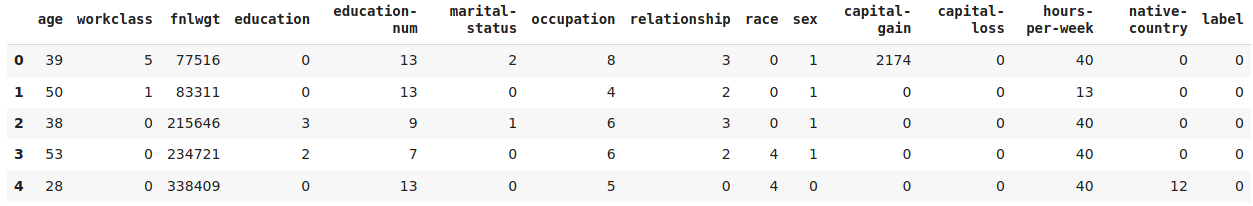
\includegraphics[scale=0.35]{df_numeric.png} 
\end{center}    

اما این روش کدگذاری داده‌های اسمی یک مشکل بزرگ دارد. برای مثال به کدگذاری متغیر relationship دقت کنید:


\begin{latin}
\begin{lstlisting}
'relationship': {'Wife':0, 'Own-child':1, 'Husband':2, 'Not-in-family':3,
                     'Other-relative':4, 'Unmarried':5},
\end{lstlisting}
\end{latin}

در این حالت به یک فرد که ازدواج نکرده‌ است عدد ۵ نسبت داده می‌شود. به یک فرد که نقش شوهر دارد عدد ۲ و به فردی که نقش زن دارد، عدد ۰، در حالی که به وضوح در دیتاست این مساله، هیچ تناسبی بین این افراد وجود ندارد. یعنی رابطه‌ای از این جهت که فرد ازدواج نکرده فاصله‌ عددش با زن یا شوهر چقدر باید باشد، وجود ندارد. \\

بنابراین از ادامه دادن مساله با این روش منصرف شده و در ادامه به سراغ روش \lr{One hot encoding} می‌رویم.

قبل از کدگذاری با استفاده از این روش، باید راه‌حلی برای داده‌های گم‌شده پیدا کنیم. در این مساله، ما برای داده‌های عددی، میانگین هر ستون را جایگزین مقدار گم‌شده کرده و برای داده‌های اسمی، مقداری که بیشترین تکرار را دارد جایگزین مقدار گم‌شده می‌کنیم. این کار با استفاده از کلاس DataFrameImputer انجام شده‌است. \\

می‌دانیم که \lr{one hot encoding} به این صورت است که به ازای هر مقدار یک متغیر، یک ستون جدید ایجاد می‌شود و ردیف‌هایی که آن مقدار را دارند، در آن ستون ۱ و در دیگر ستون‌ها مقدار ۰ خواهند گرفت. دو تابع \lr{one\_hot\_input} و \lr{one\_hot\_output} را برای تبدیل مقادیر ورودی و خروجی شبکه عصبی تعریف کرده‌ایم که در هر یک OneHotEncoder کتابخانه sklearn استفاده شده است.




% add page break after each section
\let\oldsection\section
\renewcommand\section{\clearpage\oldsection}



%%%%%%%%%%%%%%%%%%%%%%%%%%%%%%%%%%%%%%%%%%%%%%%%%%


% 2
\section{
بارگذاری داده‌ها و انجام پیش‌پردازش
}


پس از بارگذاری داده‌ها و انجام پیش‌پردازش‌های ذکرشده در بخش ۱، ستون آخر را به عنوان label در نظر گرفته و بقیه ستون‌ها را به عنوان ورودی شبکه عصبی در نظر می‌گیریم.

ابعاد ورودی و خروجی نهایی ما به صورت زیر خواهد بود:


\begin{latin}
\begin{lstlisting}
x_train_enc shape: (32561, 22141)
y_train_enc shape: (32561,)
\end{lstlisting}
\end{latin}

مجموعا ۳۲۵۶۱ داده داریم (که در آینده به عنوان داده آموزش و ارزیابی استفاده خواهد شد) و هر داده، ۲۲۱۴۱ بعد (یا ویژگی) دارد.



%%%%%%%%%%%%%%%%%%%%%%%%%%%%%%%%%%%%%%%%%%%%%%%%%%

% 3
\section{
طراحی مدل
}

برای طراحی مدل، می‌دانیم لایه ورودی، باید به اندازه شکل داده‌های ما نورون داشته باشد، بنابراین از shape متغیر \lr{x\_train\_enc} به عنوان شکل ورودی تابع استفاده می‌کنیم. همچنین می‌دانیم که در لایه آخر می‌توانیم صرفا یک نورون داشته باشیم که با یک تابع فعال‌سازی sigmoid مقدار دو کلاس را مشخص می‌کند.


%%%%%%%%%%%%%%%%%%%%%%%%%%%%%%%%%%%%%%%%%%%%%%%%%%

%\section*{منابع}

\medskip

\small
\LTR 
\latin



\end{document}
